\documentclass{standalone}
\usepackage{tikz}
\usepackage{mathrsfs}
\usetikzlibrary{positioning, shapes.geometric, arrows}
\usepackage[T1]{fontenc}
\renewcommand*\familydefault{\ttdefault} %% Only if the base font of the document is to be typewriter style
\begin{document}
	 \begin{tikzpicture}[domain=0:2,font=\small, scale=1.4]
			\draw [<->] (0,-2) -- (0,2);
			\draw [->] (0,0) -- (3,0);
			\draw (1.7,2.3) node {$y=1+\left(\dfrac{x}{2}\right)^{2}$};
			\draw(3.4,0) node {$x$};
			\draw [thick, color=red] plot(\x,{1+(\x/2)^2});
			\draw [thick, color=red] plot(\x,{-(1+(\x/2)^2)});
			\draw [thick, red] (2,0) ellipse [x radius=2,y radius=0.5, rotate=90];
		\end{tikzpicture}
\end{document}